\documentclass[10pt,twocolumn]{article}
\usepackage[margin=0.62in]{geometry}
\usepackage{amsmath,amssymb,booktabs,graphicx,microtype}
\usepackage[compact]{titlesec}
\usepackage{enumitem}
\setlist{nosep,leftmargin=*}
\titlespacing*{\section}{0pt}{0.55em}{0.25em}
\titlespacing*{\subsection}{0pt}{0.45em}{0.15em}
\setlength{\parindent}{0.8em}
\setlength{\parskip}{0pt}

\title{Selection-Channel Alignment or the Limits of Harsh Correction}
\author{Gunnar Zarncke, aintelope}
\date{May 19, 2026}

\begin{document}
\maketitle
\vspace{-1.5em}

\begin{abstract}
Robin Hanson argues that the strongest engines of cultural evolution have often been forces we morally code as ``evil'', 
such as covert politics, war, capitalism, or demographic competition. 
Moral reflection and socially praised norms drift in the absence of adaptive feedback. 
I introduce long-horizon smoothed value bundles and reified social value artifacts 
to show that selection strength alone is insufficient for value alignment.
It fails when alignment is weakened or the mechanism itself is corrupted.
\end{abstract}

\section{Why Does ``Good'' Lose?}
Hanson's ``good'' and ``evil'' are social concepts: 
``good'' names the norm-governed suppression of local competition; 
``evil'' names the competitive, covert, adversarial violation of sacredness.
The claim that latter often generate stronger selection gradients seems historically claim is plausible. 
Foragers may praise sharing but are selected for coalition skill; 
farmers may praise piety while war selects institutional forms; 
industrial society condemn capitalist selfishness while capital reallocates resources out of sight.

But a selector can be strong without being aligned (to be defined soon). 
A harsh selector may keep a culture adaptive while making it miserable. 
On the other hand, why would a strong selector be required? 
A weak selector still corrects errors, just slower. 
That is only a disadvantage if it is outcompeted by the stronger selector. But that depends on more than the strength alone.
A selector also has to maintain the memory and machinery of its corrections mechanism.
Strong selectors tend to destroy or degrade much of their machinery.
The issue is not good versus evil, nor weak versus strong selection. 
The issue is whether the correction channel remains coupled to the long-horizon bundle of human regulatory goods.
If not, even a strong selector will fail long-term.

\begin{figure*}[t]
  \centering
  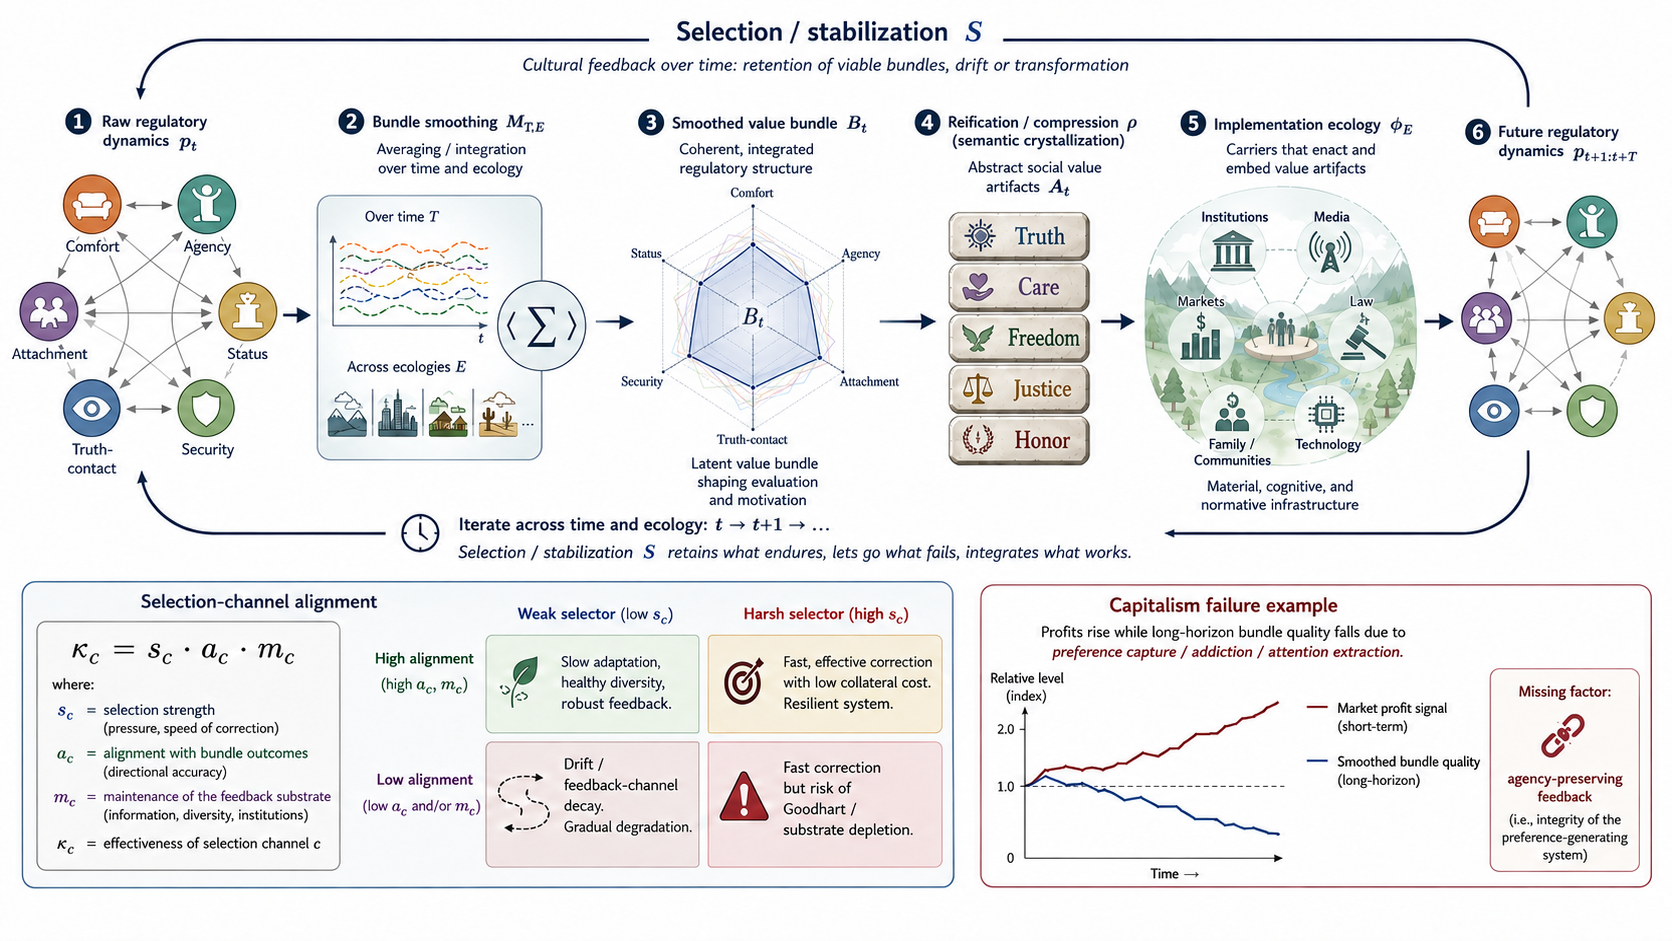
\includegraphics[width=\textwidth]{value-bundle-drift-illustration.png}
  \caption{Cultural feedback over time: raw regulatory pressures $p_t$ are smoothed into bundle $B_t$, reified as artifacts $A_t$, enacted through ecology $\phi_E$, and fed back into future dynamics. Effective correction $\kappa_c = s_c a_c m_c$ requires selection strength, bundle alignment, and substrate maintenance; weak misaligned channels drift, harsh misaligned ones Goodhart.}
  \label{fig:bundle-drift}
\end{figure*}

\section{Model}
Let $p_t$ denote a vector of raw regulatory pressures at time $t$: 
comfort, attachment, status, agency, truth-contact, novelty, threat, care, competence, and similar signals. 
These are not final values. They are local control pressures produced by human neurobiological machinery in the social environment.

Values, as modeled here, arise only after smoothing over time. Let
\begin{equation}
B_t = \mathcal M_{T,E}(p_{t:t+T})
\end{equation}
be the smoothed bundle produced by evaluating proxy trajectories over horizon $T$ in the environment $E$. 
$B_t$ is not metaphysical value; it is the regulatory pattern that is stable over longer-horizons.

Societies cannot transmit $B_t$ directly as it is the sum of what people have felt in the past. 
By reflection, communication, and agreement, they reify parts of it into value artifacts:
\begin{equation}
A_t = \rho(B_t),
\end{equation}
where these $A_t$ are compressed, transmissible, motivational representations: 
``truth'', ``care'', ``honor'', ``freedom'', ``justice'', ``good'', ``evil''. 
The quotes here reflecting Hanson's use of the communicated entitie (Good without quotes being more appropriate for the $B_t$).
The artifact then acts back on the future proxy through the environment:
\begin{equation}
A_t \xrightarrow{\phi_E} p_{t+1:t+T}.
\end{equation}

Hanson's cultural failure consists in $A$ remaining socially successful while drifting away from $B$.

\section{Hanson, Formalized}
Let $f_j(t)$ be the frequency of artifact or practice $A_j$. 
A selection channel $c$ evaluates it by some score $y_c(A_j,E)$: 
fertility, profit, military success, prestige, clicks, institutional growth, or coalition power. 
Hanson emphasizes the strength
\begin{equation}
s_c = \left|\frac{\partial \log f_j}{\partial y_c}\right|,
\end{equation}
i.e., moral culture often has low $s_c$, while war, capitalism, and demographic competition have high $s_c$; 
therefore the latter wins over the former.

But the bundle target is not $y_c$. Define the long-horizon bundle outcome
\begin{equation}
Q(A,E) = \mathcal M_{T,E}(p_{t:t+T}\mid A,E).
\end{equation}
Then the alignment of channel $c$ is approximately
\begin{equation}
a_c = \operatorname{Corr}\big(y_c(A,E), Q(A,E)\big).
\end{equation}
Finally, let $m_c$ measure mechanism maintenance: whether the selector preserves the memory, agency, trust, attention, competence, and institutional comparison structures that keep $a_c$ informative. Effective correction is not strength alone but
\begin{equation}
\kappa_c = s_c\, a_c\, m_c.
\end{equation}
This is the central correction to Hanson. A strong channel with $a_c<0$ or $m_c<0$ does not save value. It accelerates divergence.

\section{Drift vs Goodharting}
Weak correction does not fail because it stops correcting. 
It fails because \emph{other} gradients erode its mechanism. 
Long-horizon social learning depends on family transmission, intergenerational memory, local autonomy, honest comparison, survivable failure, and institutional recall. 
A culture can still notice that some practices ``do not work'', but if the memory channel is mediated by prestige, bureaucracy, media fashion, or therapy, feedback remains active while becoming less informative.

Harsh correction fails like that and not like that: War selects discipline and logistics, but also trauma, paranoia, coercion, and rulers good at war. 
Biological selection preserves fertility, but may sacrifice truth, art, mercy, education, or reflective autonomy. 
Capitalism selects responsiveness, efficiency, and innovation, but also addiction, externalities, attention capture, monopoly, and preference manipulation. 
Thus:
\begin{equation}
\text{weak selectors drift; harsh selectors Goodhart.}
\end{equation}
More precisely: weak selectors are more likely to lose memory and harsh selectors are more likely to eat their own machinery.

\section{Capitalism}
Capitalism works when price and profit track bundle-relevant constraints:
\begin{equation}
y_{\mathrm{profit}} \approx Q.
\end{equation}
It fails when profit is made by degrading the system that generates preferences. 
Addictive social media, gambling, ultra-processed food, opioids, outrage media, and some forms of pornography are not failures of correction. They are cases of rapid correction on the wrong signal. The market learns revealed preference, but the product modifies the future preference-generator. 
Then
\begin{equation}
y_{\mathrm{profit}} \uparrow \quad \text{while} \quad Q \downarrow.
\end{equation}
The missing part is not vague morality. It is the integrity of the preference-generating system: attention, agency, bodily health, trust, family stability, and reality-contact. Market selection is bundle-aligned where consumers remain competent evaluators and externalities are priced. It is bundle-divergent where products profit by reducing evaluative competence.

\section{Changing Proxy Salience}
Modern value drift need not imply rapid change in human nature. The environment changes which sub-bundles become salient:
\begin{equation}
w_i(E)=\operatorname{Salience}(p_i\mid E), \qquad p_i^{\mathrm{salient}} \xrightarrow{\rho} A_i.
\end{equation}
Scarcity and danger foreground security, kin, fertility, hierarchy, purity, and honor. 
Wealth and peace foreground autonomy, comfort, fairness, anti-domination, psychological safety, and authenticity. 
Digital attention foregrounds novelty, outrage, status comparison, identity defense, and moral display. 
The same regulatory system yields different value artifacts under different environments.

This matters because Hanson can describe modern culture as forager moral drift, but the sharper claim is domain shift: modern environments change which proxy sub-bundles are available for reflection, moralization, and institutional capture.

\section{Criterion: Substrate-Preserving Correction}
A correction mechanism is good only if it updates artifacts without corrupting the channel by which future error is detected. Formally, for plural channels $c$,
\begin{equation}
\kappa_{\mathrm{total}} = \sum_c \lambda_c s_c a_c m_c.
\end{equation}
No single channel tracks the whole bundle. Markets, law, science, family, religion, apprenticeship, democratic accountability, local communities, and technological measurement each see different parts of $Q$ and each can be captured. The engineering target is therefore not stronger selection as such, but plural, substrate-preserving, corrigible correction.

\section{Predictions}
The model predicts: (i) value artifacts selected mainly by prestige or coalition signals should semantically intensify while long-horizon bundle metrics worsen; (ii) weak cultures can still correct when memory and comparison structures remain intact; (iii) high-gradient selectors should show faster local adaptation and greater substrate depletion where externalities are available; (iv) markets whose products alter attention, agency, addiction, or trust should show profit growth with declining bundle outcomes; (v) societies with multiple semi-independent correction channels should resist both decorative moral drift and harsh-selector Goodharting better than societies dominated by one channel.

\section{Conclusion}
Hanson's strongest point is that moral praise is not an adaptive engine. The reply is that adaptive engines are not necessarily value-alignment engines. Human societies reify smoothed regulatory bundles into artifacts such as ``good'', ``evil'', ``truth'', and ``freedom''. These artifacts survive only if carried by selection channels, but those channels preserve value only when their scores remain coupled to the bundle and when they preserve the substrate that makes their own feedback informative. The future of good and evil is therefore not decided by whether culture or capitalism wins, but by whether our correction mechanisms remain aligned with the bundles they are supposed to protect.

\begin{thebibliography}{9}\setlength{\itemsep}{0pt}
\bibitem{hanson2026} Hanson, R. (2026). \emph{The Past and Future of Good and Evil}. Overcoming Bias.
\end{thebibliography}

\end{document}
